\FChapter{Chapter Thirty-Seven}{37}

\Lettrine{T}{he} \textsc{manor-house} of Ferndean was a building of considerable antiquity,
moderate size, and no architectural pretensions, deep buried in a wood.
I had heard of it before. \Mr{} Rochester often spoke of it, and
sometimes went there. His father had purchased the estate for the sake
of the game covers. He would have let the house, but could find no
tenant, in consequence of its ineligible and insalubrious site.
Ferndean then remained uninhabited and unfurnished, with the exception
of some two or three rooms fitted up for the accommodation of the squire
when he went there in the season to shoot.

To this house I came just ere dark on an evening marked by the
characteristics of sad sky, cold gale, and continued small penetrating
rain. The last mile I performed on foot, having dismissed the chaise
and driver with the double remuneration I had promised. Even when
within a very short distance of the manor-house, you could see nothing
of it, so thick and dark grew the timber of the gloomy wood about it.
Iron gates between granite pillars showed me where to enter, and passing
through them, I found myself at once in the twilight of close-ranked
trees. There was a grass-grown track descending the forest aisle
between hoar and knotty shafts and under branched arches. I followed
it, expecting soon to reach the dwelling; but it stretched on and on, it
wound far and farther: no sign of habitation or grounds was visible.

I thought I had taken a wrong direction and lost my way. The darkness
of natural as well as of sylvan dusk gathered over me. I looked round
in search of another road. There was none: all was interwoven stem,
columnar trunk, dense summer foliage---no opening anywhere.

I proceeded: at last my way opened, the trees thinned a little;
presently I beheld a railing, then the house---scarce, by this dim
light, distinguishable from the trees; so dank and green were its
decaying walls. Entering a portal, fastened only by a latch, I stood
amidst a space of enclosed ground, from which the wood swept away in a
semicircle. There were no flowers, no garden-beds; only a broad
gravel-walk girdling a grass-plat, and this set in the heavy frame of
the forest. The house presented two pointed gables in its front; the
windows were latticed and narrow: the front door was narrow too, one
step led up to it. The whole looked, as the host of the Rochester Arms
had said, \enquote{quite a desolate spot.} It was as still as a church
on a week-day: the pattering rain on the forest leaves was the only
sound audible in its vicinage.

\enquote{Can there be life here?} I asked.

Yes, life of some kind there was; for I heard a movement---that narrow
front-door was unclosing, and some shape was about to issue from the
grange.

It opened slowly: a figure came out into the twilight and stood on the
step; a man without a hat: he stretched forth his hand as if to feel
whether it rained. Dusk as it was, I had recognised him---it was my
master, Edward Fairfax Rochester, and no other.

I stayed my step, almost my breath, and stood to watch him---to examine
him, myself unseen, and alas! to him invisible. It was a sudden
meeting, and one in which rapture was kept well in check by pain. I had
no difficulty in restraining my voice from exclamation, my step from
hasty advance.

His form was of the same strong and stalwart contour as ever: his port
was still erect, his hair was still raven black; nor were his features
altered or sunk: not in one year's space, by any sorrow, could his
athletic strength be quelled or his vigorous prime blighted. But in his
countenance I saw a change: that looked desperate and brooding---that
reminded me of some wronged and fettered wild beast or bird, dangerous
to approach in his sullen woe. The caged eagle, whose gold-ringed eyes
cruelty has extinguished, might look as looked that sightless Samson.

And, reader, do you think I feared him in his blind ferocity?---if you
do, you little know me. A soft hope blest with my sorrow that soon I
should dare to drop a kiss on that brow of rock, and on those lips so
sternly sealed beneath it: but not yet. I would not accost him yet.

He descended the one step, and advanced slowly and gropingly towards the
grass-plat. Where was his daring stride now? Then he paused, as if he
knew not which way to turn. He lifted his hand and opened his eyelids;
gazed blank, and with a straining effort, on the sky, and toward the
amphitheatre of trees: one saw that all to him was void darkness. He
stretched his right hand (the left arm, the mutilated one, he kept
hidden in his bosom); he seemed to wish by touch to gain an idea of what
lay around him: he met but vacancy still; for the trees were some yards
off where he stood. He relinquished the endeavour, folded his arms, and
stood quiet and mute in the rain, now falling fast on his uncovered
head. At this moment John approached him from some quarter.

\enquote{Will you take my arm, sir?} he said; \enquote{there is a heavy
	shower coming on: had you not better go in?}

\enquote{Let me alone,} was the answer.

John withdrew without having observed me. \Mr{} Rochester now tried to
walk about: vainly,---all was too uncertain. He groped his way back to
the house, and, re-entering it, closed the door.

I now drew near and knocked: John's wife opened for me. \enquote{Mary,}
I said, \enquote{how are you?}

She started as if she had seen a ghost: I calmed her. To her hurried
\enquote{Is it really you, miss, come at this late hour to this lonely
	place?} I answered by taking her hand; and then I followed her into the
kitchen, where John now sat by a good fire. I explained to them, in few
words, that I had heard all which had happened since I left Thornfield,
and that I was come to see \Mr{} Rochester. I asked John to go down to
the turn-pike-house, where I had dismissed the chaise, and bring my
trunk, which I had left there: and then, while I removed my bonnet and
shawl, I questioned Mary as to whether I could be accommodated at the
Manor House for the night; and finding that arrangements to that effect,
though difficult, would not be impossible, I informed her I should
stay. Just at this moment the parlour-bell rang.

\enquote{When you go in,} said I, \enquote{tell your master that a
	person wishes to speak to him, but do not give my name.}

\enquote{I don't think he will see you,} she answered; \enquote{he
	refuses everybody.}

When she returned, I inquired what he had said. \enquote{You are to
	send in your name and your business,} she replied. She then proceeded
to fill a glass with water, and place it on a tray, together with
candles.

\enquote{Is that what he rang for?} I asked.

\enquote{Yes: he always has candles brought in at dark, though he is
	blind.}

\enquote{Give the tray to me; I will carry it in.}

I took it from her hand: she pointed me out the parlour door. The tray
shook as I held it; the water spilt from the glass; my heart struck my
ribs loud and fast. Mary opened the door for me, and shut it behind me.

This parlour looked gloomy: a neglected handful of fire burnt low in the
grate; and, leaning over it, with his head supported against the high,
old-fashioned mantelpiece, appeared the blind tenant of the room. His
old dog, Pilot, lay on one side, removed out of the way, and coiled up
as if afraid of being inadvertently trodden upon. Pilot pricked up his
ears when I came in: then he jumped up with a yelp and a whine, and
bounded towards me: he almost knocked the tray from my hands. I set it
on the table; then patted him, and said softly, \enquote{Lie down!} \Mr{}
Rochester turned mechanically to \emph{see} what the commotion was: but
as he \emph{saw} nothing, he returned and sighed.

\enquote{Give me the water, Mary,} he said.

I approached him with the now only half-filled glass; Pilot followed me,
still excited.

\enquote{What is the matter?} he inquired.

\enquote{Down, Pilot!} I again said. He checked the water on its way to
his lips, and seemed to listen: he drank, and put the glass down.
\enquote{This is you, Mary, is it not?}

\enquote{Mary is in the kitchen,} I answered.

He put out his hand with a quick gesture, but not seeing where I stood,
he did not touch me. \enquote{Who is this? Who is this?} he demanded,
trying, as it seemed, to \emph{see} with those sightless
eyes---unavailing and distressing attempt! \enquote{Answer me---speak
	again!} he ordered, imperiously and aloud.

\enquote{Will you have a little more water, sir? I spilt half of what
	was in the glass,} I said.

\enquote{\emph{Who} is it? \emph{What} is it? Who speaks?}

\enquote{Pilot knows me, and John and Mary know I am here. I came only
	this evening,} I answered.

\enquote{Great God!---what delusion has come over me? What sweet
	madness has seized me?}

\enquote{No delusion---no madness: your mind, sir, is too strong for
	delusion, your health too sound for frenzy.}

\enquote{And where is the speaker? Is it only a voice? Oh! I \emph{cannot}
	see, but I must feel, or my heart will stop and my brain burst.
	Whatever---whoever you are---be perceptible to the touch or I cannot
	live!}

He groped; I arrested his wandering hand, and prisoned it in both mine.

\enquote{Her very fingers!} he cried; \enquote{her small, slight
	fingers! If so there must be more of her.}

The muscular hand broke from my custody; my arm was seized, my
shoulder---neck---waist---I was entwined and gathered to him.

\enquote{Is it Jane? \emph{What} is it? This is her shape---this is her
	size---}

\enquote{And this her voice,} I added. \enquote{She is all here: her
	heart, too. God bless you, sir! I am glad to be so near you again.}

\enquote{Jane Eyre!---Jane Eyre,} was all he said.

\enquote{My dear master,} I answered, \enquote{I am Jane Eyre: I have
	found you out---I am come back to you.}

\enquote{In truth?---in the flesh? My living Jane?}

\enquote{You touch me, sir,---you hold me, and fast enough: I am not
	cold like a corpse, nor vacant like air, am I?}

\enquote{My living darling! These are certainly her limbs, and these
	her features; but I cannot be so blest, after all my misery. It is a
	dream; such dreams as I have had at night when I have clasped her once
	more to my heart, as I do now; and kissed her, as thus---and felt that
	she loved me, and trusted that she would not leave me.}

\enquote{Which I never will, sir, from this day.}

\enquote{Never will, says the vision? But I always woke and found it an
	empty mockery; and I was desolate and abandoned---my life dark, lonely,
	hopeless---my soul athirst and forbidden to drink---my heart famished
	and never to be fed. Gentle, soft dream, nestling in my arms now, you
	will fly, too, as your sisters have all fled before you: but kiss me
	before you go---embrace me, Jane.}

\enquote{There, sir---and there!}'

I pressed my lips to his once brilliant and now rayless eyes---I swept
his hair from his brow, and kissed that too. He suddenly seemed to
arouse himself: the conviction of the reality of all this seized him.

\enquote{It is you---is it, Jane? You are come back to me then?}

\enquote{I am.}

\enquote{And you do not lie dead in some ditch under some stream? And
	you are not a pining outcast amongst strangers?}

\enquote{No, sir! I am an independent woman now.}

\enquote{Independent! What do you mean, Jane?}

\enquote{My uncle in Madeira is dead, and he left me five thousand
	pounds.}

\enquote{Ah! this is practical---this is real!} he cried: \enquote{I
	should never dream that. Besides, there is that peculiar voice of hers,
	so animating and piquant, as well as soft: it cheers my withered heart;
	it puts life into it.---What, Janet! Are you an independent woman? A
	rich woman?}

\enquote{If you won't let me live with you, I can build a house of my
	own close up to your door, and you may come and sit in my parlour when
	you want company of an evening.}

\enquote{But as you are rich, Jane, you have now, no doubt, friends who
	will look after you, and not suffer you to devote yourself to a blind
	lameter like me?}

\enquote{I told you I am independent, sir, as well as rich: I am my own
	mistress.}

\enquote{And you will stay with me?}

\enquote{Certainly---unless you object. I will be your neighbour, your
	nurse, your housekeeper. I find you lonely: I will be your
	companion---to read to you, to walk with you, to sit with you, to wait
	on you, to be eyes and hands to you. Cease to look so melancholy, my
	dear master; you shall not be left desolate, so long as I live.}

He replied not: he seemed serious---abstracted; he sighed; he
half-opened his lips as if to speak: he closed them again. I felt a
little embarrassed. Perhaps I had too rashly over-leaped
conventionalities; and he, like \St{} John, saw impropriety in my
inconsiderateness. I had indeed made my proposal from the idea that he
wished and would ask me to be his wife: an expectation, not the less
certain because unexpressed, had buoyed me up, that he would claim me at
once as his own. But no hint to that effect escaping him and his
countenance becoming more overcast, I suddenly remembered that I might
have been all wrong, and was perhaps playing the fool unwittingly; and I
began gently to withdraw myself from his arms---but he eagerly snatched
me closer.

\enquote{No---no---Jane; you must not go. No---I have touched you,
	heard you, felt the comfort of your presence---the sweetness of your
	consolation: I cannot give up these joys. I have little left in
	myself---I must have you. The world may laugh---may call me absurd,
	selfish---but it does not signify. My very soul demands you: it will be
	satisfied, or it will take deadly vengeance on its frame.}

\enquote{Well, sir, I will stay with you: I have said so.}

\enquote{Yes---but you understand one thing by staying with me; and I
	understand another. You, perhaps, could make up your mind to be about
	my hand and chair---to wait on me as a kind little nurse (for you have
	an affectionate heart and a generous spirit, which prompt you to make
	sacrifices for those you pity), and that ought to suffice for me no
	doubt. I suppose I should now entertain none but fatherly feelings for
	you: do you think so? Come---tell me.}

\enquote{I will think what you like, sir: I am content to be only your
	nurse, if you think it better.}

\enquote{But you cannot always be my nurse, Janet: you are young---you
	must marry one day.}

\enquote{I don't care about being married.}

\enquote{You should care, Janet: if I were what I once was, I would try
	to make you care---but---a sightless block!}

He relapsed again into gloom. I, on the contrary, became more cheerful,
and took fresh courage: these last words gave me an insight as to where
the difficulty lay; and as it was no difficulty with me, I felt quite
relieved from my previous embarrassment. I resumed a livelier vein of
conversation.

\enquote{It is time some one undertook to rehumanise you,} said I,
parting his thick and long uncut locks; \enquote{for I see you are being
	metamorphosed into a lion, or something of that sort. You have a
	\enquote{faux air} of Nebuchadnezzar in the fields about you, that is
	certain: your hair reminds me of eagles' feathers; whether your nails
	are grown like birds' claws or not, I have not yet noticed.}

\enquote{On this arm, I have neither hand nor nails,} he said, drawing
the mutilated limb from his breast, and showing it to me. \enquote{It
	is a mere stump---a ghastly sight! Don't you think so, Jane?}

\enquote{It is a pity to see it; and a pity to see your eyes---and the
	scar of fire on your forehead: and the worst of it is, one is in danger
	of loving you too well for all this; and making too much of you.}

\enquote{I thought you would be revolted, Jane, when you saw my arm, and
	my cicatrised visage.}

\enquote{Did you? Don't tell me so---lest I should say something
	disparaging to your judgment. Now, let me leave you an instant, to make
	a better fire, and have the hearth swept up. Can you tell when there is
	a good fire?}

\enquote{Yes; with the right eye I see a glow---a ruddy haze.}

\enquote{And you see the candles?}

\enquote{Very dimly---each is a luminous cloud.}

\enquote{Can you see me?}

\enquote{No, my fairy: but I am only too thankful to hear and feel you.}

\enquote{When do you take supper?}

\enquote{I never take supper.}

\enquote{But you shall have some to-night. I am hungry: so are you, I
	daresay, only you forget.}

Summoning Mary, I soon had the room in more cheerful order: I prepared
him, likewise, a comfortable repast. My spirits were excited, and with
pleasure and ease I talked to him during supper, and for a long time
after. There was no harassing restraint, no repressing of glee and
vivacity with him; for with him I was at perfect ease, because I knew I
suited him; all I said or did seemed either to console or revive him.
Delightful consciousness! It brought to life and light my whole nature:
in his presence I thoroughly lived; and he lived in mine. Blind as he
was, smiles played over his face, joy dawned on his forehead: his
lineaments softened and warmed.

After supper, he began to ask me many questions, of where I had been,
what I had been doing, how I had found him out; but I gave him only very
partial replies: it was too late to enter into particulars that night.
Besides, I wished to touch no deep-thrilling chord---to open no fresh
well of emotion in his heart: my sole present aim was to cheer him.
Cheered, as I have said, he was: and yet but by fits. If a moment's
silence broke the conversation, he would turn restless, touch me, then
say, \enquote{Jane.}

\enquote{You are altogether a human being, Jane? You are certain of
	that?}

\begin{figure}
	\begin{sidecaption}{\enquote{You are altogether a\linebreak human being, Jane?\linebreak You are certain of that?}}[p422b]
		\centering
		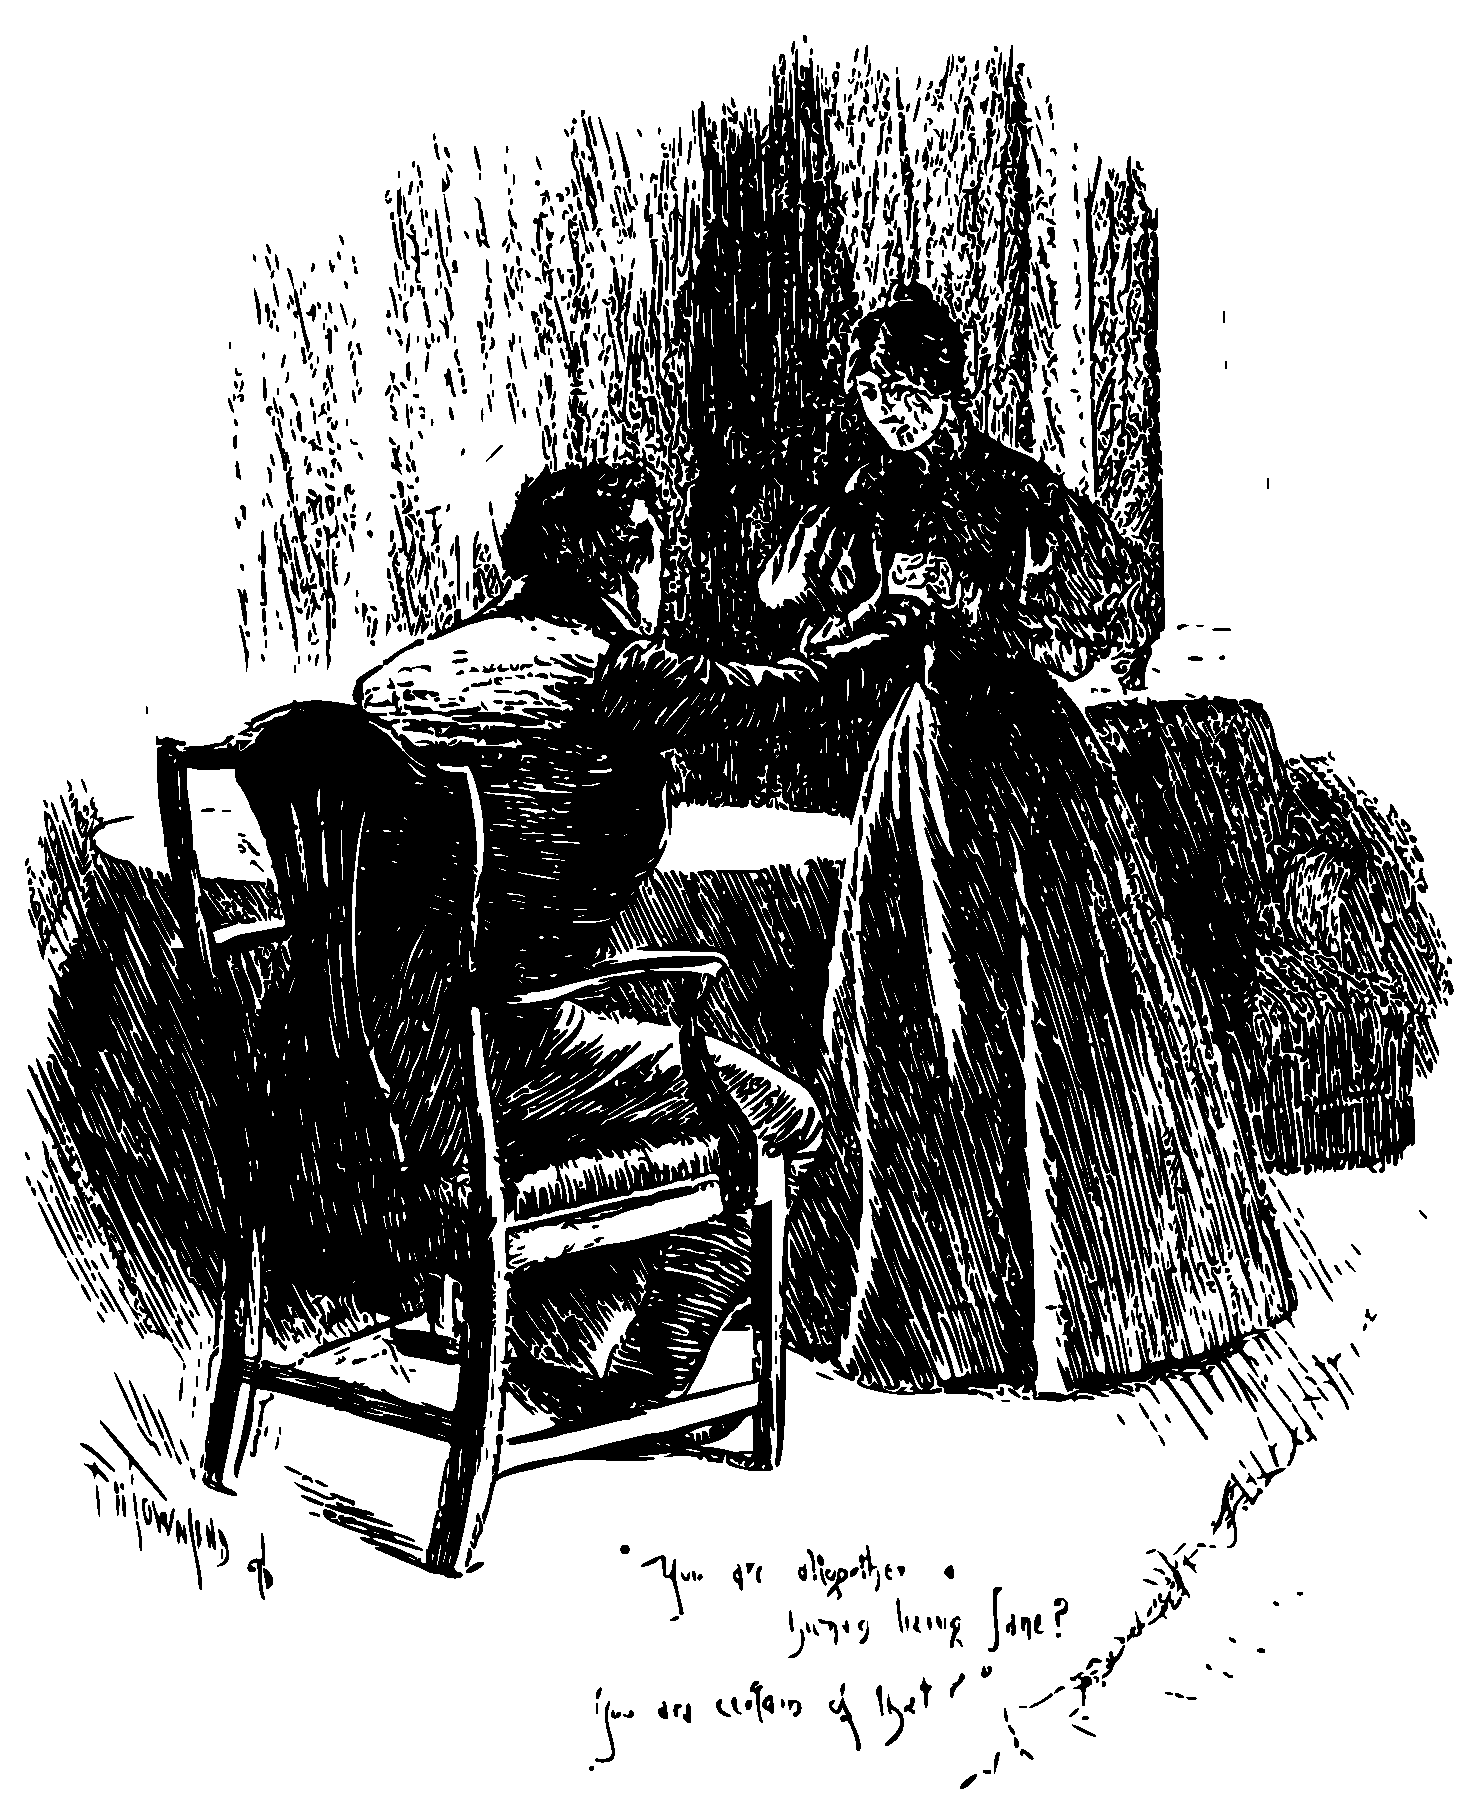
\includegraphics[width=\linewidth]{images/p422b.pdf}
	\end{sidecaption}
\end{figure}

\enquote{I conscientiously believe so, \Mr{} Rochester.}

\enquote{Yet how, on this dark and doleful evening, could you so
	suddenly rise on my lone hearth? I stretched my hand to take a glass of
	water from a hireling, and it was given me by you: I asked a question,
	expecting John's wife to answer me, and your voice spoke at my ear.}

\enquote{Because I had come in, in Mary's stead, with the tray.}

\enquote{And there is enchantment in the very hour I am now spending
	with you. Who can tell what a dark, dreary, hopeless life I have
	dragged on for months past? Doing nothing, expecting nothing; merging
	night in day; feeling but the sensation of cold when I let the fire go
	out, of hunger when I forgot to eat: and then a ceaseless sorrow, and,
	at times, a very delirium of desire to behold my Jane again. Yes: for
	her restoration I longed, far more than for that of my lost sight. How
	can it be that Jane is with me, and says she loves me? Will she not
	depart as suddenly as she came? To-morrow, I fear I shall find her no
	more.}

A commonplace, practical reply, out of the train of his own disturbed
ideas, was, I was sure, the best and most reassuring for him in this
frame of mind. I passed my finger over his eyebrows, and remarked that
they were scorched, and that I would apply something which would make
them grow as broad and black as ever.

\enquote{Where is the use of doing me good in any way, beneficent spirit, when,
	at some fatal moment, you will again desert me---passing like a shadow,
	whither and how to me unknown, and for me remaining afterwards
	undiscoverable?} %fix missing end quote

\enquote{Have you a pocket-comb about you, sir?}

\enquote{What for, Jane?}

\enquote{Just to comb out this shaggy black mane. I find you rather
	alarming, when I examine you close at hand: you talk of my being a
	fairy, but I am sure, you are more like a brownie.}

\enquote{Am I hideous, Jane?}

\enquote{Very, sir: you always were, you know.}

\enquote{Humph! The wickedness has not been taken out of you, wherever
	you have sojourned.}

\enquote{Yet I have been with good people; far better than you: a
	hundred times better people; possessed of ideas and views you never
	entertained in your life: quite more refined and exalted.}

\enquote{Who the deuce have you been with?}

\enquote{If you twist in that way you will make me pull the hair out of
	your head; and then I think you will cease to entertain doubts of my
	substantiality.}

\enquote{Who have you been with, Jane?}

\enquote{You shall not get it out of me to-night, sir; you must wait
	till to-morrow; to leave my tale half told, will, you know, be a sort of
	security that I shall appear at your breakfast table to finish it. By
	the bye, I must mind not to rise on your hearth with only a glass of
	water then: I must bring an egg at the least, to say nothing of fried
	ham.}

\enquote{You mocking changeling---fairy-born and human-bred! You make
	me feel as I have not felt these twelve months. If Saul could have had
	you for his David, the evil spirit would have been exorcised without the
	aid of the harp.}

\enquote{There, sir, you are redd up and made decent. Now I'll leave
	you: I have been travelling these last three days, and I believe I am
	tired. Good night.}

\enquote{Just one word, Jane: were there only ladies in the house where
	you have been?}

I laughed and made my escape, still laughing as I ran upstairs.
\enquote{A good idea!} I thought with glee. \enquote{I see I have the
	means of fretting him out of his melancholy for some time to come.}

Very early the next morning I heard him up and astir, wandering from one
room to another. As soon as Mary came down I heard the question:
\enquote{Is Miss Eyre here?} Then: \enquote{Which room did you put her
	into? Was it dry? Is she up? Go and ask if she wants anything; and
	when she will come down.}

I came down as soon as I thought there was a prospect of breakfast.
Entering the room very softly, I had a view of him before he discovered
my presence. It was mournful, indeed, to witness the subjugation of
that vigorous spirit to a corporeal infirmity. He sat in his
chair---still, but not at rest: expectant evidently; the lines of now
habitual sadness marking his strong features. His countenance reminded
one of a lamp quenched, waiting to be re-lit---and alas! it was not
himself that could now kindle the lustre of animated expression: he was
dependent on another for that office! I had meant to be gay and
careless, but the powerlessness of the strong man touched my heart to
the quick: still I accosted him with what vivacity I could.

\enquote{It is a bright, sunny morning, sir,} I said. \enquote{The rain
	is over and gone, and there is a tender shining after it: you shall have
	a walk soon.}

I had wakened the glow: his features beamed.

\enquote{Oh, you are indeed there, my skylark! Come to me. You are not
	gone: not vanished? I heard one of your kind an hour ago, singing high
	over the wood: but its song had no music for me, any more than the
	rising sun had rays. All the melody on earth is concentrated in my
	Jane's tongue to my ear (I am glad it is not naturally a silent one):
	all the sunshine I can feel is in her presence.}

The water stood in my eyes to hear this avowal of his dependence; just
as if a royal eagle, chained to a perch, should be forced to entreat a
sparrow to become its purveyor. But I would not be lachrymose: I dashed
off the salt drops, and busied myself with preparing breakfast.

Most of the morning was spent in the open air. I led him out of the wet
and wild wood into some cheerful fields: I described to him how
brilliantly green they were; how the flowers and hedges looked
refreshed; how sparklingly blue was the sky. I sought a seat for him in
a hidden and lovely spot, a dry stump of a tree; nor did I refuse to let
him, when seated, place me on his knee. Why should I, when both he and
I were happier near than apart? Pilot lay beside us: all was quiet. He
broke out suddenly while clasping me in his arms---

\enquote{Cruel, cruel deserter! Oh, Jane, what did I feel when I
	discovered you had fled from Thornfield, and when I could nowhere find
	you; and, after examining your apartment, ascertained that you had taken
	no money, nor anything which could serve as an equivalent! A pearl
	necklace I had given you lay untouched in its little casket; your trunks
	were left corded and locked as they had been prepared for the bridal
	tour. What could my darling do, I asked, left destitute and penniless?
	And what did she do? Let me hear now.}

Thus urged, I began the narrative of my experience for the last year. I
softened considerably what related to the three days of wandering and
starvation, because to have told him all would have been to inflict
unnecessary pain: the little I did say lacerated his faithful heart
deeper than I wished.

I should not have left him thus, he said, without any means of making my
way: I should have told him my intention. I should have confided in
him: he would never have forced me to be his mistress. Violent as he
had seemed in his despair, he, in truth, loved me far too well and too
tenderly to constitute himself my tyrant: he would have given me half
his fortune, without demanding so much as a kiss in return, rather than
I should have flung myself friendless on the wide world. I had endured,
he was certain, more than I had confessed to him.

\enquote{Well, whatever my sufferings had been, they were very short,} I
answered: and then I proceeded to tell him how I had been received at
Moor House; how I had obtained the office of schoolmistress, \etc. The
accession of fortune, the discovery of my relations, followed in due
order. Of course, \St{} John Rivers' name came in frequently in the
progress of my tale. When I had done, that name was immediately taken
up.

\enquote{This \St{} John, then, is your cousin?}

\enquote{Yes.}

\enquote{You have spoken of him often: do you like him?}

\enquote{He was a very good man, sir; I could not help liking him.}

\enquote{A good man. Does that mean a respectable well-conducted man of
	fifty? Or what does it mean?}

\enquote{St John was only twenty-nine, sir.}

\enquote{\foreignquote{french}{\emph{Jeune encore,}}\footnote{young again} as the French say. Is he a person of low
	stature, phlegmatic, and plain. A person whose goodness consists rather
	in his guiltlessness of vice, than in his prowess in virtue.}

\enquote{He is untiringly active. Great and exalted deeds are what he
	lives to perform.}

\enquote{But his brain? That is probably rather soft? He means well:
	but you shrug your shoulders to hear him talk?}

\enquote{He talks little, sir: what he does say is ever to the point.
	His brain is first-rate, I should think not impressible, but vigorous.}

\enquote{Is he an able man, then?}

\enquote{Truly able.}

\enquote{A thoroughly educated man?}

\enquote{\St{} John is an accomplished and profound scholar.}

\enquote{His manners, I think, you said are not to your
	taste?---priggish and parsonic?}

\enquote{I never mentioned his manners; but, unless I had a very bad
	taste, they must suit it; they are polished, calm, and gentlemanlike.}

\enquote{His appearance,---I forget what description you gave of his
	appearance;---a sort of raw curate, half strangled with his white
	neckcloth, and stilted up on his thick-soled high-lows, eh?}

\enquote{\St{} John dresses well. He is a handsome man: tall, fair, with
	blue eyes, and a Grecian profile.}

(Aside.) \enquote{Damn him!}---(To me.) \enquote{Did you like him,
	Jane?}

\enquote{Yes, \Mr{} Rochester, I liked him: but you asked me that before.}

I perceived, of course, the drift of my interlocutor. Jealousy had got
hold of him: she stung him; but the sting was salutary: it gave him
respite from the gnawing fang of melancholy. I would not, therefore,
immediately charm the snake.

\enquote{Perhaps you would rather not sit any longer on my knee, Miss
	Eyre?} was the next somewhat unexpected observation.

\enquote{Why not, \Mr{} Rochester?}

\enquote{The picture you have just drawn is suggestive of a rather too
	overwhelming contrast. Your words have delineated very prettily a
	graceful Apollo: he is present to your imagination,---tall, fair,
	blue-eyed, and with a Grecian profile. Your eyes dwell on a Vulcan,---a
	real blacksmith, brown, broad-shouldered: and blind and lame into the
	bargain.}

\enquote{I never thought of it, before; but you certainly are rather
	like Vulcan, sir.}

\enquote{Well, you can leave me, ma'am: but before you go} (and he
retained me by a firmer grasp than ever), \enquote{you will be pleased
	just to answer me a question or two.} He paused.

\enquote{What questions, \Mr{} Rochester?}

Then followed this cross-examination.

\enquote{\St{} John made you schoolmistress of Morton before he knew you
	were his cousin?}

\enquote{Yes.}

\enquote{You would often see him? He would visit the school sometimes?}

\enquote{Daily.}

\enquote{He would approve of your plans, Jane? I know they would be
	clever, for you are a talented creature!}

\enquote{He approved of them---yes.}

\enquote{He would discover many things in you he could not have expected
	to find? Some of your accomplishments are not ordinary.}

\enquote{I don't know about that.}

\enquote{You had a little cottage near the school, you say: did he ever
	come there to see you?}

\enquote{Now and then?}

\enquote{Of an evening?}

\enquote{Once or twice.}

A pause.

\enquote{How long did you reside with him and his sisters after the
	cousinship was discovered?}

\enquote{Five months.}

\enquote{Did Rivers spend much time with the ladies of his family?}

\enquote{Yes; the back parlour was both his study and ours: he sat near
	the window, and we by the table.}

\enquote{Did he study much?}

\enquote{A good deal.}

\enquote{What?}

\enquote{Hindostanee.}

\enquote{And what did you do meantime?}

\enquote{I learnt German, at first.}

\enquote{Did he teach you?}

\enquote{He did not understand German.}

\enquote{Did he teach you nothing?}

\enquote{A little Hindostanee.}

\enquote{Rivers taught you Hindostanee?}

\enquote{Yes, sir.}

\enquote{And his sisters also?}

\enquote{No.}

\enquote{Only you?}

\enquote{Only me.}

\enquote{Did you ask to learn?}

\enquote{No.}

\enquote{He wished to teach you?}

\enquote{Yes.}

A second pause.

\enquote{Why did he wish it? Of what use could Hindostanee be to you?}

\enquote{He intended me to go with him to India.}

\enquote{Ah! here I reach the root of the matter. He wanted you to
	marry him?}

\enquote{He asked me to marry him.}

\enquote{That is a fiction---an impudent invention to vex me.}

\enquote{I beg your pardon, it is the literal truth: he asked me more
	than once, and was as stiff about urging his point as ever you could
	be.}

\enquote{Miss Eyre, I repeat it, you can leave me. How often am I to
	say the same thing? Why do you remain pertinaciously perched on my
	knee, when I have given you notice to quit?}

\enquote{Because I am comfortable there.}

\enquote{No, Jane, you are not comfortable there, because your heart is
	not with me: it is with this cousin---this \St{} John. Oh, till this
	moment, I thought my little Jane was all mine! I had a belief she loved
	me even when she left me: that was an atom of sweet in much bitter.
	Long as we have been parted, hot tears as I have wept over our
	separation, I never thought that while I was mourning her, she was
	loving another! But it is useless grieving. Jane, leave me: go and
	marry Rivers.}

\enquote{Shake me off, then, sir,---push me away, for I'll not leave you
	of my own accord.}

\enquote{Jane, I ever like your tone of voice: it still renews hope, it
	sounds so truthful. When I hear it, it carries me back a year. I
	forget that you have formed a new tie. But I am not a fool---go---}

\enquote{Where must I go, sir?}

\enquote{Your own way---with the husband you have chosen.}

\enquote{Who is that?}

\enquote{You know---this \St{} John Rivers.}

\enquote{He is not my husband, nor ever will be. He does not love me: I do not
	love him. He loves (as he \emph{can} love, and that is not as you love)
	a beautiful young lady called Rosamond. He wanted to marry me only
	because he thought I should make a suitable missionary's wife, which she
	would not have done. He is good and great, but severe; and, for me,
	cold as an iceberg. He is not like you, sir: I am not happy at his
	side, nor near him, nor with him. He has no indulgence for me---no
	fondness. He sees nothing attractive in me; not even youth---only a few
	useful mental points.---Then I must leave you, sir, to go to him?}

I shuddered involuntarily, and clung instinctively closer to my blind
but beloved master. He smiled.

\enquote{What, Jane! Is this true? Is such really the state of matters
	between you and Rivers?}

\enquote{Absolutely, sir! Oh, you need not be jealous! I wanted to tease you
	a little to make you less sad: I thought anger would be better than
	grief. But if you wish me to love you, could you but see how much I
	\emph{do} love you, you would be proud and content. All my heart is
	yours, sir: it belongs to you; and with you it would remain, were fate
	to exile the rest of me from your presence for ever.}

Again, as he kissed me, painful thoughts darkened his aspect.

\enquote{My seared vision! My crippled strength!} he murmured
regretfully.

I caressed, in order to soothe him. I knew of what he was thinking, and
wanted to speak for him, but dared not. As he turned aside his face a
minute, I saw a tear slide from under the sealed eyelid, and trickle
down the manly cheek. My heart swelled.

\enquote{I am no better than the old lightning-struck chestnut-tree in
	Thornfield orchard,} he remarked ere long. \enquote{And what right
	would that ruin have to bid a budding woodbine cover its decay with
	freshness?}

\enquote{You are no ruin, sir---no lightning-struck tree: you are green
	and vigorous. Plants will grow about your roots, whether you ask them
	or not, because they take delight in your bountiful shadow; and as they
	grow they will lean towards you, and wind round you, because your
	strength offers them so safe a prop.}

Again he smiled: I gave him comfort.

\enquote{You speak of friends, Jane?} he asked.

\enquote{Yes, of friends,} I answered rather hesitatingly: for I knew I
meant more than friends, but could not tell what other word to employ.
He helped me.

\enquote{Ah! Jane. But I want a wife.}

\enquote{Do you, sir?}

\enquote{Yes: is it news to you?}

\enquote{Of course: you said nothing about it before.}

\enquote{Is it unwelcome news?}

\enquote{That depends on circumstances, sir---on your choice.}

\enquote{Which you shall make for me, Jane. I will abide by your
	decision.}

\enquote{Choose then, sir---\emph{her who loves you best}.}

\enquote{I will at least choose---\emph{her I love best}. Jane, will you marry
	me?}

\enquote{Yes, sir.}

\enquote{A poor blind man, whom you will have to lead about by the
	hand?}

\enquote{Yes, sir.}

\enquote{A crippled man, twenty years older than you, whom you will have
	to wait on?}

\enquote{Yes, sir.}

\enquote{Truly, Jane?}

\enquote{Most truly, sir.}

\enquote{Oh! my darling! God bless you and reward you!}

\enquote{\Mr{} Rochester, if ever I did a good deed in my life---if ever I
	thought a good thought---if ever I prayed a sincere and blameless
	prayer---if ever I wished a righteous wish,---I am rewarded now. To be
	your wife is, for me, to be as happy as I can be on earth.}

\enquote{Because you delight in sacrifice.}

\enquote{Sacrifice! What do I sacrifice? Famine for food, expectation
	for content. To be privileged to put my arms round what I value---to
	press my lips to what I love---to repose on what I trust: is that to
	make a sacrifice? If so, then certainly I delight in sacrifice.}

\enquote{And to bear with my infirmities, Jane: to overlook my
	deficiencies.}

\enquote{Which are none, sir, to me. I love you better now, when I can
	really be useful to you, than I did in your state of proud independence,
	when you disdained every part but that of the giver and protector.}

\enquote{Hitherto I have hated to be helped---to be led: henceforth, I
	feel I shall hate it no more. I did not like to put my hand into a
	hireling's, but it is pleasant to feel it circled by Jane's little
	fingers. I preferred utter loneliness to the constant attendance of
	servants; but Jane's soft ministry will be a perpetual joy. Jane suits
	me: do I suit her?}

\enquote{To the finest fibre of my nature, sir.}

\enquote{The case being so, we have nothing in the world to wait for: we
	must be married instantly.}

He looked and spoke with eagerness: his old impetuosity was rising.

\enquote{We must become one flesh without any delay, Jane: there is but
	the licence to get---then we marry.}

\enquote{\Mr{} Rochester, I have just discovered the sun is far declined
	from its meridian, and Pilot is actually gone home to his dinner. Let
	me look at your watch.}

\enquote{Fasten it into your girdle, Janet, and keep it henceforward: I
	have no use for it.}

\enquote{It is nearly four o'clock in the afternoon, sir. Don't you
	feel hungry?}

\enquote{The third day from this must be our wedding-day, Jane. Never
	mind fine clothes and jewels, now: all that is not worth a fillip.}

\enquote{The sun has dried up all the rain-drops, sir. The breeze is
	still: it is quite hot.}

\enquote{Do you know, Jane, I have your little pearl necklace at this
	moment fastened round my bronze scrag under my cravat? I have worn it
	since the day I lost my only treasure, as a memento of her.}

\enquote{We will go home through the wood: that will be the shadiest
	way.}

He pursued his own thoughts without heeding me.

\enquote{Jane! you think me, I daresay, an irreligious dog: but my heart swells
	with gratitude to the beneficent God of this earth just now. He sees
	not as man sees, but far clearer: judges not as man judges, but far more
	wisely. I did wrong: I would have sullied my innocent flower---breathed
	guilt on its purity: the Omnipotent snatched it from me. I, in my
	stiff-necked rebellion, almost cursed the dispensation: instead of
	bending to the decree, I defied it. Divine justice pursued its course;
	disasters came thick on me: I was forced to pass through the valley of
	the shadow of death. \emph{His} chastisements are mighty; and one smote
	me which has humbled me for ever. You know I was proud of my strength:
	but what is it now, when I must give it over to foreign guidance, as a
	child does its weakness? Of late, Jane---only---only of late---I began
	to see and acknowledge the hand of God in my doom. I began to
	experience remorse, repentance; the wish for reconcilement to my Maker.
	I began sometimes to pray: very brief prayers they were, but very
	sincere.

	%rem enq
	Some days since: nay, I can number them---four; it was last Monday
	night, a singular mood came over me: one in which grief replaced
	frenzy---sorrow, sullenness. I had long had the impression that since I
	could nowhere find you, you must be dead. Late that night---perhaps it
	might be between eleven and twelve o'clock---ere I retired to my dreary
	rest, I supplicated God, that, if it seemed good to Him, I might soon be
	taken from this life, and admitted to that world to come, where there
	was still hope of rejoining Jane.

	%rem enq
	I was in my own room, and sitting by the window, which was
	open: it soothed me to feel the balmy night-air; though I could see no
	stars and only by a vague, luminous haze, knew the presence of a moon.
	I longed for thee, Janet! Oh, I longed for thee both with soul and
	flesh! I asked of God, at once in anguish and humility, if I had not
	been long enough desolate, afflicted, tormented; and might not soon
	taste bliss and peace once more. That I merited all I endured, I
	acknowledged---that I could scarcely endure more, I pleaded; and the
	alpha and omega of my heart's wishes broke involuntarily from my lips in
	the words---\enquote{Jane! Jane! Jane!}}

\enquote{Did you speak these words aloud?}

\enquote{I did, Jane. If any listener had heard me, he would have
	thought me mad: I pronounced them with such frantic energy.}

\enquote{And it was last Monday night, somewhere near midnight?}

\enquote{Yes; but the time is of no consequence: what followed is the strange
	point. You will think me superstitious,---some superstition I have in
	my blood, and always had: nevertheless, this is true---true at least it
	is that I heard what I now relate.

	%rem enq
	As I exclaimed \enquote{Jane! Jane! Jane!} a voice---I cannot tell
	whence the voice came, but I know whose voice it was---replied,
	\enquote{I am coming: wait for me;} and a moment after, went whispering
	on the wind the words---\enquote{Where are you?}

	%rem enq
	I'll tell you, if I can, the idea, the picture these words
	opened to my mind: yet it is difficult to express what I want to
	express. Ferndean is buried, as you see, in a heavy wood, where sound
	falls dull, and dies unreverberating. \enquote{Where are you?} seemed
	spoken amongst mountains; for I heard a hill-sent echo repeat the
	words. Cooler and fresher at the moment the gale seemed to visit my
	brow: I could have deemed that in some wild, lone scene, I and Jane were
	meeting. In spirit, I believe we must have met. You no doubt were, at
	that hour, in unconscious sleep, Jane: perhaps your soul wandered from
	its cell to comfort mine; for those were your accents---as certain as I
	live---they were yours!}

Reader, it was on Monday night---near midnight---that I too had received
the mysterious summons: those were the very words by which I replied to
it. I listened to \Mr{} Rochester's narrative, but made no disclosure in
return. The coincidence struck me as too awful and inexplicable to be
communicated or discussed. If I told anything, my tale would be such as
must necessarily make a profound impression on the mind of my hearer:
and that mind, yet from its sufferings too prone to gloom, needed not
the deeper shade of the supernatural. I kept these things then, and
pondered them in my heart.

\enquote{You cannot now wonder,} continued my master, \enquote{that when
	you rose upon me so unexpectedly last night, I had difficulty in
	believing you any other than a mere voice and vision, something that
	would melt to silence and annihilation, as the midnight whisper and
	mountain echo had melted before. Now, I thank God! I know it to be
	otherwise. Yes, I thank God!}

He put me off his knee, rose, and reverently lifting his hat from his
brow, and bending his sightless eyes to the earth, he stood in mute
devotion. Only the last words of the worship were audible.

\enquote{I thank my Maker, that, in the midst of judgment, he has
	remembered mercy. I humbly entreat my Redeemer to give me strength to
	lead henceforth a purer life than I have done hitherto!}

Then he stretched his hand out to be led. I took that dear hand, held
it a moment to my lips, then let it pass round my shoulder: being so
much lower of stature than he, I served both for his prop and guide. We
entered the wood, and wended homeward.
